\chapter{Analysis}
\label{cap:methods}
\section{Similarity}
    To measure similarity in the neural activity in different trials, we used the Mahalanobis Distance \eqref{eqn:mahalanobis}. For two vectors $\vec{u}$ and $\vec{v}$, and covariance $\Sigma$:
    \begin{equation}
        \quad D_m(\vec{u},\vec{v}) = \sqrt{(\vec{u}-\vec{v})^T\Sigma^{-1}(\vec{u}-\vec{v})}
        \label{eqn:mahalanobis}
    \end{equation}
    We calculate the covariance matrices using 'oas' shrinkage \cite{chen2010shrinkage}, recalculating at each split, and using a different covariance matrix for each time step.
    \vskip1ex
    \begin{algorithm}[H]
     \KwData{Firing\_rates, 3d array of shape $(n_t, n_{\eta}, n_k)$}
     \KwResult{D, 2d array of distances, shape $(n_t, n_t)$ }
     \For{iter = 1 to 1000}{
          half$^{(1)}$, half$^{(2)}$ <- split(Firing\_rates) %into two $(n_t, n_{\eta},\frac{n_k}{2})$ halfs;
          
            \For{t = 1 to $n_t$}{
            $\mu_t^{(1)}$ = mean(half$^{(1)}_t$, along='trials'  )\\
            $\mu_t^{(2)}$ = mean(half$^{(2)}_t$, along='trials'  )\\
            resid = concatenate(half$^{(1)}_t$ -  $\mu_t^{(1)}$,  half$^{(2)}_t$ -  $\mu_t^{(2)}$)\\
            $\Sigma_{t}$ = cov(resid)
            }
        \For{i,j in \textit{combinations}($n_t, n_t$)}{
            $D^{iter}(i,j) = \frac{1}{2}\sqrt{\mu_i^{(1)}\Sigma_{i}^{-1}\mu_j^{(2)}} +
             		  \frac{1}{2}\sqrt{\mu_i^{(1)}\Sigma_{j}^{-1}\mu_j^{(2)}}$
        }
     }
     $D$ = mean($D^{iter}$, along='iter')
     
     \caption{Mahalanobis similarity}
     
    \end{algorithm}
    \vskip1ex
    We split the trials in two halves $k_1$, $k_2$ \footnote{e.g. $k_1=[1,2,5,7,...]$, $k2=[3,4,6,8,...]$}, took the mean activity of each partition along trial axis $\mu^1=\left<F^{k_1}\right>$ and measured the pairwise distances between times across partition. That is, the distance between times $i$ and $j$ measured in one single split is:
    \begin{equation*}
        \frac{1}{2} \left[ D(\mu^1_{t=i},\mu^2_{t=j} ) + D(\mu^1_{t=j},\mu^2_{t=i}) \right]
        %\label{eqn:split}
    \end{equation*}
    
    This process was repeated 1000 times with different random splits of the trials, and the mean distance for each pair of times defines a distance matrix. The grand distance is the mean across subjects of their distance matrix. We applied measures of depth \cite{mosler2013depth} to measure similarity between time points. Put simply, the similarity (or depth) S is calculated for a distance metric D as 
    \begin{equation*}
    S = \frac{1}{1+D}
    \label{eqn:depth}
    \end{equation*}

\section{Machine learning}
    Following the literature\cite{bakhurin2017differential}, we treated the problem as one of classification, in which each time bin is given a label, and a model is trained to find the right label for each data point. In other words, we use the instantaneous firing rate of all neurons to predict how much time has passed since the animal inserted its nose.
    
    \subsection{Metrics}
    Following Bakhurin et al \cite{bakhurin2017differential}, we evaluated models using the Pearson's correlation \eqref{eqn:pearson} between expected and predicted labels $x$ and $y$. 
    % In addition, in some cases we measure accuracy \eqref{eqn:acc} and Cohen's kappa\eqref{eqn:kappa}.
    
    % \begin{equation}
    %     Accuracy \quad  :=  \quad \frac{\sum_{i=1}^N\delta(T_i,P_i)}{N}
    %     \label{eqn:acc}
    % \end{equation}
    
    \begin{equation}
        Pearson's\quad r  \quad :=  \quad
            \frac{Cov(x,y)}{\sqrt{Var(x)Var(y)}}
        \label{eqn:pearson}
    \end{equation}
    
    % \begin{equation}
    %     Cohen's \quad \kappa  \quad :=  \quad 1-  \frac{\sum_{i=1}^k\sum_{j=1}^kw_{ij}x_{ij}}{\sum_{i=1}^k\sum_{j=1}^kw_{ij}m_{ij}}
    %     \label{eqn:kappa}
    % \end{equation}
    
    % \subsection{Cross-validation}
    We evaluated models using Monte Carlo cross validation, which means we generated multiple random splits of the data for training, and evaluated the predictions on the remainder of each split. 

    \subsection{Classifier selection and hyperparameter tuning}
        In the classifier comparison, to find good hyperparameters for each classifier, we applied a bayesian search using the scikit-optimization library \cite{skopt}. This procedure begins by randomly searching the parameter space, and after some iterations it starts to make estimates of the function values in the parameter space, sampling points with high estimated value. The fit of hyperparameter space is done by gausian processes, and its implementation is dealt with entirely by the library. The length of search was defined for each classifier depending on the number of hyperparameters to tune.%, and is available along with hyperparameters chosen to optimize in the annex. % TODO annex
        
        We have compared a total of 12 different classifiers, all of them from out-of-the-box implementations in python libraries. Of these classifiers, 10 were taken from the scikit-learn \cite{scikit-learn} library, while two of them, XGBoost \cite{chen2016xgboost} and LightGBM \cite{ke2017lightgbm}, were taken from their own libraries, both having an api similar to sklearn's.

    \subsection{Comparison of time representation}
        For one set of animals we had long sessions of more than 1000 trials $(1149 \pm 384)$ with sufficient correct trials $(660 \pm 260)$, and in this case we split correct trials into first and second half. For the second set of animals, in which sessions were half as long with $570 \pm 181$ trials and $284\pm 100$ correct ones, we instead compared correct trials in the first versus second session. Then we measured classification performance in each using Logistic Regression. 
        
        % ramping: We applied a one-vs-rest Logistic Regression classifier, that evaluates N different classifiers for the N labels, combining all their outputs to give the probability of each label given the data point. We have not tuned hyperparameters, using L2 regularization with the default value of C=1. We used 50 shuffles of monte-carlo cross validation to measure classifier's performance, ensuring that points from the same trial were always jointly assigned, in each shuffle choosing 80\% of the data points to fit the model and the remaining to evaluate it. We evaluated the performance using pearson's correlation between true and predicted labels. In the ramping neurons performance comparison, we hold constant the number of features in each (14), by randomly choosing 14 non-ramping neurons in each split, while using all 14 ramping neurons. Probability matrices are calculated by taking the average output probability of all datapoints of each label. 
        % \subsection{LSTM} quem sabe para a defesa
        
        % This process is generally made in several steps, by first filtering the signal, then selecting the spikes by thresholding, reducing dimensionality of the spikes, clustering the spikes and finally by assigning scores to each cluster, that measure the degree of confidence that those spikes are really from a neuron's action potentials, as opposed to noise \cite{}. These steps can be performed by spike-sorting softwares, in which user interaction is minimal, such as waveclus \cite{}
        
        %colocar imagem de esqueminha

\section{Rationale}
    \begin{figure}
        \centering
        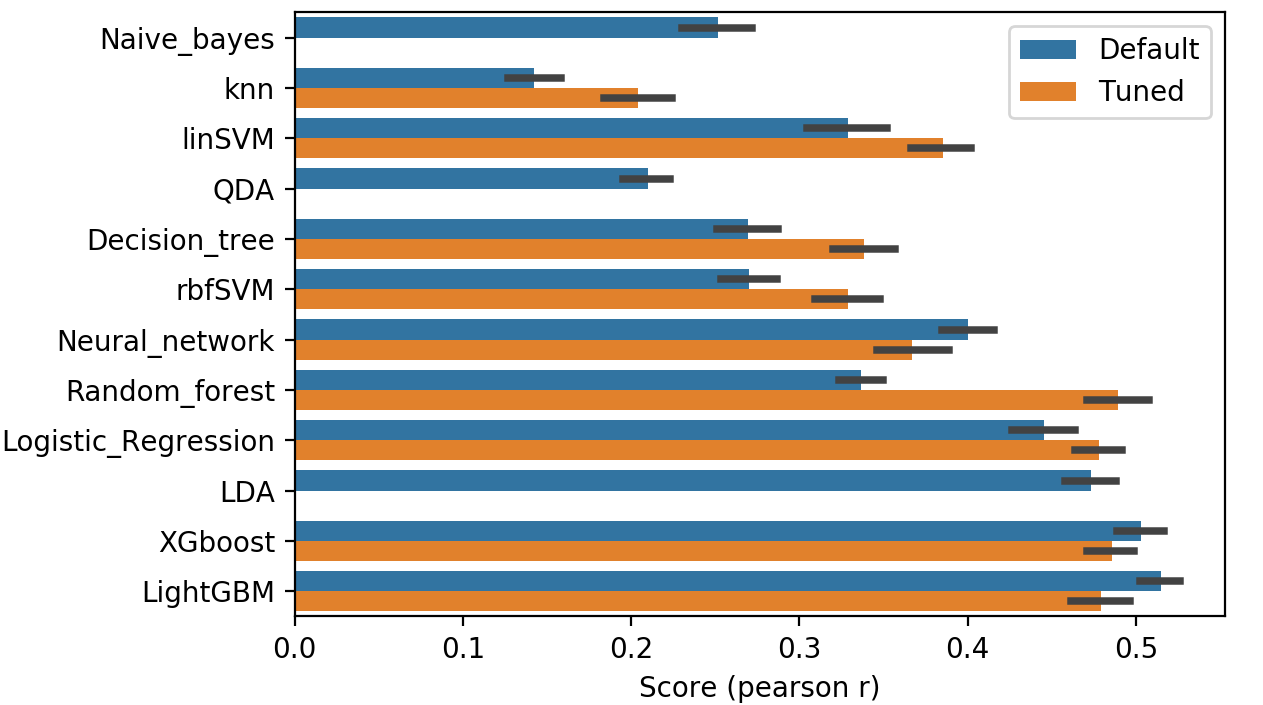
\includegraphics[width=\textwidth]{figures/clf_comparison.png}
        \caption[Comparison of classifiers]{Comparison of classifiers. Default hyperparameters were compared with those resulting from tuning when there were hyperparameters to tune.}
        \label{fig:clf_comparison}
    \end{figure} % Mean performance+-SEM for each classifier tuned and untuned. 
    Firstly, we compared classification performances for different classifiers, in such a way as to make an informed choice for our subsequent analysis. We calculate scores in each tuning step with 5 folds of Monte Carlo cross validation, and evaluate the final scores with 50 folds. Half of the trials were hold out for tuning, trials from the other half were used for evaluation of the final score.
    
    We found big differences in performance between the multiple classifiers tested. Some classifiers have good results out-of-the-box, such as Logistic Regression and Linear Discriminant Analysis (LDA), while some are highly dependent on hyperparameter tuning, such as Random Forest. The results for the gradient boosting classifiers LightGBM and XGBoost are specially interesting, as they have better results on the default configurations than after tuning, which is probably due to the fact that we were tuning 10 different hyperparameters, making us prone to overfitting the tuning.
    
    \begin{figure}
        \centering
        % \includegraphics[width=\textwidth]{figuras/methods/learning_curves_sppfc.png}
        \caption{Classifier learning curves}
        \label{fig:clf_curves}
    \end{figure}
    % Colocar aqui somente para os melhores. Colocar os outros no material suplementar.
    For most classifiers, there is significant decoding for as little as 10 trials in the training set. As expected, the classifier's performance increases with the number of trials used for training it. It is even possible that a bigger training set would give us even higher scores, pointing to the importance of having big experimental sessions with many trials. Hence, if we want to compare the information contained in the neural activity in different moments in a session, we have to ensure their classification models are trained with the same number of trials.
